\documentclass[border=3pt,tikz]{standalone}
\usepackage{amsmath}
%\usetikzlibrary{calc}
%\usetikzlibrary{decorations.pathmorphing} % for snakes
\usetikzlibrary {shapes.geometric} % for star
\usetikzlibrary{bending} % for arrow head angle
\usetikzlibrary{angles,quotes} % for pic (angle labels)
\usetikzlibrary{arrows.meta} % for arrow size

\usetikzlibrary {3d} 
\usetikzlibrary {arrows}
\usetikzlibrary{shapes.geometric}
\begin{document}
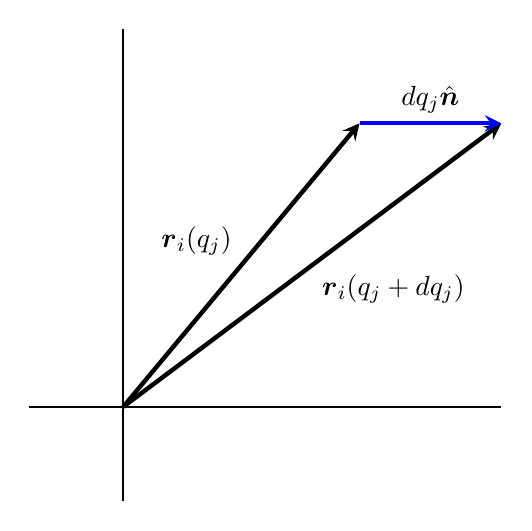
\begin{tikzpicture}[scale=1.2, rotate=0]
    \coordinate (O) at (0,0);
    \coordinate (A) at (4,0);
    \coordinate (B) at (0,4);
    \coordinate (R1) at (2.5,3);
    \coordinate (R2) at (4,3);
    \draw[thick] (-1,0) -- (A);
    \draw[thick] (0,-1) -- (B);
    \draw[-stealth, ultra thick] (O) -- (R1);
    \draw[-stealth, ultra thick] (O) -- (R2);
    \draw[-stealth, ultra thick, blue] (R1) -- (R2);
    \node [anchor=south east] at (1.25,1.5) {$\boldsymbol{r}_i(q_j)$};
    \node [anchor=north west] at (2,1.5) {$\boldsymbol{r}_i(q_j+dq_j)$};
    \node [anchor=south ] at (3.25,3) {$dq_j\hat{\boldsymbol{n}}$};
  \end{tikzpicture}
\end{document}